% This work is licensed under the Creative Commons Attribution NonCommercial
% ShareAlike 4.0 International License. To view a copy of the license, visit
% https://creativecommons.org/licenses/by-nc-sa/4.0/

\documentclass[twoside,10pt]{book}
\usepackage[T1]{fontenc}
\usepackage[utf8]{inputenc}
\usepackage{import}

% Typography -------------------------------------------------------------------
\usepackage{newtxtext}
\usepackage[lining]{FiraSans}
\usepackage{inconsolata}
\usepackage{amsmath,amssymb,amsfonts}
\usepackage{bm}
\usepackage[american]{babel}
\usepackage[protrusion=true,factor=900]{microtype}
\usepackage{ccicons}

% Page geometry, page, part, chapter, and section styles -----------------------
% This work is licensed under the Creative Commons Attribution NonCommercial
% ShareAlike 4.0 International License. To view a copy of the license, visit
% https://creativecommons.org/licenses/by-nc-sa/4.0/

\usepackage{calc}
\usepackage[
  paperwidth=16cm,paperheight=24cm,
  body={118mm,185mm},
  %hmarginratio=25:17,
  hcentering,
  vcentering,
  headsep=2pc]{geometry}

\usepackage[pagestyles,explicit,clearempty]{titlesec}
\usepackage{xcolor}
\usepackage{pagecolor}
\usepackage{afterpage}
\usepackage{tikz}
\usetikzlibrary{arrows}
\usetikzlibrary{calc}

\definecolor{gray0}{RGB}{154,154,154}
\definecolor{gray1}{RGB}{204,204,204}
\definecolor{gray2}{RGB}{235,235,235}

\definecolor{red1}{RGB}{239,71,111}
\definecolor{yellow1}{RGB}{255,209,102}
\definecolor{green1}{RGB}{5,171,128}
\definecolor{blue1}{RGB}{17,138,178}
\definecolor{violet1}{RGB}{7,59,76}

\colorlet{red0}{red1!80!black}
\colorlet{red2}{red1!80!white}
\colorlet{yellow0}{yellow1!80!black}
\colorlet{yellow2}{yellow1!80!white}
\colorlet{green0}{green1!80!black}
\colorlet{green2}{green1!80!white}
\colorlet{blue0}{blue1!80!black}
\colorlet{blue2}{blue1!80!white}
\colorlet{violet0}{violet1!80!black}
\colorlet{violet2}{violet1!80!white}

\definecolor{covercolor}{RGB}{23,40,81}
\colorlet{titlescolor}{blue0}

\newpagestyle{chapter}{
  \setfoot
  [\normalfont\sffamily\color{titlescolor}\bfseries\thepage][][]
  {}{}{\normalfont\sffamily\color{titlescolor}\bfseries\thepage}
  \settitlemarks{part,chapter}
}

\renewpagestyle{plain}{
  \sethead
  [\normalfont\sffamily\color{titlescolor}
    \ifthechapter
      {{\bfseries
      \MakeUppercase{\chaptertitlename}~\thechapter}\quad\chaptertitle}
      {\ifthenelse{\not\equal{\thepart}{}}
        {{\bfseries PART~\thepart}\quad\parttitle}
        {}}][][]
  {}{}{\normalfont\sffamily\color{titlescolor}
    \ifthechapter
      {{\bfseries\thesection}\quad\sectiontitle}
      {\ifthenelse{\not\equal{\thepart}{}}
        {{\bfseries PART~\thepart}\quad\parttitle}
        {}}}
  \setfoot
  [\normalfont\sffamily\color{titlescolor}\bfseries\thepage][][]
  {}{}{\normalfont\sffamily\color{titlescolor}\bfseries\thepage}
  \settitlemarks{part,chapter}
}

\assignpagestyle{\part}{empty}
\assignpagestyle{\chapter}{chapter}
\pagestyle{plain}

\newlength{\partnumberwidth}
\newlength{\parttitlesep}
\setlength{\partnumberwidth}{2.4cm}
\setlength{\parttitlesep}{6mm}
\titleformat{\part}[block]{}{}{0pt}{
  \thispagestyle{empty}
  \begin{tikzpicture}
    \scope[inner xsep=0, outer sep=0, align=center, text=titlescolor]
    \node (number) [
    anchor=north east,
    text width=\partnumberwidth]
    {\fontsize{115}{115}\selectfont\thepart};
    \node[
    anchor=south east,
    outer ysep=\parttitlesep,
    text width=\partnumberwidth,
    text=white,fill=titlescolor]
    at (node cs:name=number, anchor=north east)
    {\sffamily\fontsize{18}{18}\fontseries{bx}\selectfont PART};
    \node [
    anchor=north west,
    inner xsep=\parttitlesep,
    text width=0.99\linewidth - \partnumberwidth - 2\parttitlesep,
    align=flush left]
    at (node cs:name=number, anchor=north east)
    {\sffamily\fontsize{32}{40}\fontseries{l}\selectfont#1\\};
    \endscope
  \end{tikzpicture}
}

\newlength{\chapternumberwidth}
\newlength{\chaptertitlesep}
\setlength{\chapternumberwidth}{2cm}
\setlength{\chaptertitlesep}{3mm}
\titleformat{\chapter}[block]{}{}{0pt}{
  \begin{tikzpicture}
    \scope[inner xsep=0, outer sep=0, align=center, text=titlescolor]
    \node (number) [
    minimum width=\chapternumberwidth]
    {\fontsize{84}{84}\selectfont\thechapter};
    \path let \p1=(number.west), \p2=(number.east) in
    node[
    anchor=south east,
    outer ysep=\chaptertitlesep,
    text width=\x2-\x1,
    text=white,fill=titlescolor]
    at (node cs:name=number, anchor=north east)
    {\sffamily\fontseries{bx}\selectfont \MakeUppercase{\chaptertitlename}};
    \path let \p1=(number.west), \p2=(number.east) in
    node [
    anchor=north west,
    inner xsep=\chaptertitlesep,
    text width=0.99\linewidth - (\x2 - \x1) - 2\chaptertitlesep,
    align=flush left]
    at (node cs:name=number, anchor=north east)
    {\sffamily\fontsize{22}{28}\fontseries{l}\selectfont#1\\};
    \endscope
  \end{tikzpicture}
}

\titleformat{name=\chapter,numberless}
  {\color{titlescolor}}
  {}
  {0mm}
  {\sffamily\fontsize{22}{28}\fontseries{l}\selectfont#1\\}

\titleformat{\section}
  {\Large\sffamily\bfseries\color{titlescolor}}
  {\thesection}{8pt}{#1}

\titleformat{\subsection}
  {\large\sffamily\bfseries\color{titlescolor}}
  {\thesubsection}{8pt}{#1}

\titleformat{\subsubsection}
  {\normalsize\sffamily\bfseries\color{titlescolor}}
  {\thesubsubsection}{8pt}{#1}

\titleformat{\paragraph}[runin]
  {\normalsize\sffamily\bfseries}{}{0pt}{#1}

\titlespacing*{\chapter}{0mm}{0mm}{1pc}
\titlespacing*{\section}{0mm}{5.3mm}{2.1mm}
\titlespacing*{\subsection}{0mm}{5.3mm}{2.1mm}
\titlespacing*{\subsubsection}{0mm}{4.2mm}{1.1mm}
\titlespacing*{\paragraph}{0mm}{0mm}{2mm}

\usepackage{titletoc}
\usepackage[nottoc]{tocbibind}

\titlecontents{part}
[0em]
{\vspace{1cm}\normalfont\sffamily\bfseries\fontsize{14}{16}\selectfont}
{}
{\color{titlescolor}PART }
{\titlerule*[0.7pc]{.}\normalfont\small\sffamily\selectfont\contentspage}
[\vspace{3mm}]

\titlecontents{chapter}
[0em]
{\normalfont\sffamily\bfseries\fontsize{12}{16}\selectfont}
{\color{titlescolor}\MakeUppercase{\chaptertitlename}
 {\thecontentslabel}\hspace{4mm}}
{}
{\titlerule*[0.7pc]{.}\normalfont\small\sffamily\selectfont\contentspage}

\titlecontents{section}
[0em]
{\normalfont\normalsize\selectfont}
{\color{titlescolor}\sffamily\bfseries\fontsize{10}{12}\selectfont%
  \makebox[12mm][r]{\thecontentslabel}%
  \hspace{2mm}\normalfont\normalsize\selectfont}
{}
{\titlerule*[0.7pc]{.}\normalfont\small\sffamily\selectfont\contentspage}

\newcommand\appendixintoc{\def\chaptertitlename{\appendixname}}



% Paragraph styles (spacing, lists, single and multicolums) --------------------
% This work is licensed under the Creative Commons Attribution NonCommercial
% ShareAlike 4.0 International License. To view a copy of the license, visit
% https://creativecommons.org/licenses/by-nc-sa/4.0/

\newenvironment{Paragraph}[1][\bigskip]%
  {#1\noindent\ignorespaces}%
  {\unskip\bigskip}

\usepackage{enumitem}
\setlist{noitemsep}
\setlist[itemize]{leftmargin=*,label={$\bullet$}}
\setlist[enumerate]{leftmargin=*}

\usepackage{multicol}
\setlength{\columnsep}{4.5mm}
\newlength{\defaultcolumnsep}
\setlength{\defaultcolumnsep}{\columnsep}

\newenvironment{TwoColumns}
  {\setlength{\columnsep}{0.8cm}%
   \setlength{\columnseprule}{0.4pt}%
   \begin{multicols}{2}}
  {\end{multicols}%
   \setlength{\columnsep}{\defaultcolumnsep}%
   \setlength{\columnseprule}{0pt}}

\usepackage{paracol}
\setcolumnwidth{,5.5cm}




% Verbatim and highlighting styles for source code listings --------------------
% This work is licensed under the Creative Commons Attribution NonCommercial
% ShareAlike 4.0 International License. To view a copy of the license, visit
% https://creativecommons.org/licenses/by-nc-sa/4.0/

\usepackage{framed}
\colorlet{shadecolor}{yellow1!10!white}
\newenvironment{Shaded}{\setlength\topsep{0pt}\begin{snugshade}\small}
  {\end{snugshade}}

\usepackage{fancyvrb}
\DefineVerbatimEnvironment{Highlighting}{Verbatim}{}

\DefineVerbatimEnvironment{Code}{Verbatim}
  {commandchars=\\\{\},fontsize=\small}

\newlength{\ColorBoxWidth}%
\newcommand{\ColorBox}[2]%
{%
  \settowidth{\ColorBoxWidth}{#2}%
  \setlength{\fboxsep}{0pt}%
  \raisebox{0.1\baselineskip}[0pt][0pt]{%
    \colorbox{#1}{\parbox[c][\baselineskip]{\ColorBoxWidth}{~}}%
  }%
  \hspace{-\ColorBoxWidth}#2%
}
\colorlet{Inserted}{green1!10!white}
\colorlet{Deleted}{red1!10!white}
\newcommand{\ToyComment}[1]{\textcolor{gray}{#1}}
\newcommand{\ToyConst}[1]{\textcolor{gray}{#1}}
\newcommand{\ToyParam}[1]{\textcolor{gray}{#1}}
\newcommand{\ToyVar}[1]{\textcolor{gray}{#1}}
\newcommand{\ToyLet}[1]{\textcolor{gray}{\makebox[1.5em]{$\rightarrow$}{#1}}}
\newcommand{\ToyDelete}[1]{\ColorBox{Deleted}{#1}}
\newcommand{\ToyInsert}[1]{\ColorBox{Inserted}{#1}}
\newcommand{\ToyWrap}{\textcolor{gray}{\makebox[0.5em]{$\wr$}}}
\newcommand{\ToyUnwrap}{\textcolor{gray}{\makebox[0.5em]{$\wr$}}}
\newcommand{\ToyChange}{\rlap{\hspace{-5pt}%
    \raisebox{-0.2\baselineskip}[0pt][0pt]{\rule{1pt}{\baselineskip}}}}


% Figure, table, and algorithm styles ------------------------------------------
% This work is licensed under the Creative Commons Attribution NonCommercial
% ShareAlike 4.0 International License. To view a copy of the license, visit
% https://creativecommons.org/licenses/by-nc-sa/4.0/

\usepackage{dpfloat}
\usepackage{caption}

% Figures ---------------------------------------------------------------------

\newenvironment{Figure}[1][tbp]%
  {\begin{figure}[#1]\sffamily\small\centering}%
  {\end{figure}}

\DeclareCaptionFont{figlabelfont}{\small\color{titlescolor}}
\DeclareCaptionFont{figcaptionfont}{\small}
\captionsetup[figure]{
  labelsep=quad,
  labelfont={figlabelfont,bf,sf},
  font={figcaptionfont,sf},
  name=FIGURE,
}

% Tables ----------------------------------------------------------------------

\usepackage{longtable}
\usepackage{makecell}
\renewcommand\theadfont{\bfseries}
\renewcommand\theadalign{l}
\renewcommand\theadgape{}
\renewcommand\cellalign{l}
\renewcommand\cellgape{\Gape[2pt][0pt]}

\newenvironment{Table}[1][tbp]%
  {\begin{table}[#1]\sffamily\small\centering}%
  {\end{table}}

\captionsetup[table]{
  labelsep=quad,
  labelfont={figlabelfont,bf,sf},
  font={figcaptionfont,sf},
  name=TABLE,
}

% Algorithms ------------------------------------------------------------------

\usepackage[chapter]{algorithm}
\usepackage{algorithmicx}

% Fix some pdflatex warnings, see https://tex.stackexchange.com/questions/177025
\newcounter{Halgorithmic}
\AtBeginEnvironment{algorithmic}{\stepcounter{Halgorithmic}}
\ExpandArgs{c}\newcommand{theHALG@line}{\arabic{Halgorithmic}.\arabic{ALG@line}}

\algdef{SN}[DefaultBlock]{Begin}{End}{}
\algdef{CN}[ContinueBlock]{DefaultBlock}{Continue}{End}{}
\renewcommand\alglinenumber[1]{\footnotesize #1.}
\renewcommand\algorithmicindent{1em}

\newenvironment{Algorithm}[1][tbp]%
  {\begin{algorithm}[#1]}%
  {\end{algorithm}}

\captionsetup[algorithm]{
  labelsep=quad,
  labelfont={figlabelfont,bf,sf},
  font={figcaptionfont,sf},
  name=ALGORITHM,
}



% Hyperlinks, cross references and URLs ----------------------------------------
% This work is licensed under the Creative Commons Attribution NonCommercial
% ShareAlike 4.0 International License. To view a copy of the license, visit
% https://creativecommons.org/licenses/by-nc-sa/4.0/

\usepackage[unicode]{hyperref}
\usepackage{bookmark}
\usepackage[noabbrev,capitalize]{cleveref}
\usepackage{xurl}
\usepackage{latexgit}

\urlstyle{same}

\hypersetup{
  bookmarksnumbered=true,
  colorlinks=true,
  allcolors=titlescolor,
  pdftitle={Programming a toy computer from scratch},
  pdfauthor={Eric Bruneton},
  pdflang={en},
}

\newcommand{\raisedhypertarget}[1]
  {\raisebox{\baselineskip}[0pt]{\hypertarget{#1}{}}}

\newcommand{\toypcurl}[1]{\url{https://ebruneton.github.io/toypc/#1}}


% Commands for literate programming --------------------------------------------
% The Latex code is preprocessed with a Rust program. This produces some
% generated Rust files, which are then run. In turn, these generated Rust files
% generate some Latex files, which are finally \input in the main Latex files.
% This work is licensed under the Creative Commons Attribution NonCommercial
% ShareAlike 4.0 International License. To view a copy of the license, visit
% https://creativecommons.org/licenses/by-nc-sa/4.0/

\newcommand{\rustfile}{}
\newcounter{rustid}
\globalcounter{rustid}

% The preprocessor appends the content of this command to a generated Rust
% source file 'book/src/part<x>/chapter<y>_generator.rs'.
\newcommand{\rust}[1]{}

% The preprocessor appends to the above generated Rust source file some
% instructions to evaluate the content of this command, which must be a Rust
% expression. These instructions then save the value of this expression in
% 'book/part<x>/generated/chapter<y>_input<z>.tex', which is finally '\input'
% in the Latex file using this command.
\newcommand{\rs}[1]{%
  \input{generated/\rustfile/input\therustid.tex}\unskip%
  \addtocounter{rustid}{1}%
}

% The preprocessor appends the content of this command to the above generated
% Rust source file. These must be instructions using a BytecodeAssembler
% object. The result of these instructions is automatically saved in
% 'book/part<x>/generated/chapter<y>_input<z>.tex', with the
% BytecodeAssembler::write method, using as options the optional argument of
% this command. This generated file is finally '\input' in the Latex file using
% this command.
\newcommand{\bytecode}[2][]{%
  \input{generated/\rustfile/input\therustid.tex}\unskip%
  \addtocounter{rustid}{1}%
}

% The preprocessor appends the content of this command to the above generated
% Rust source file. This content must be source code which can be parsed by a
% Transpiler object. It is added line by line with the Transpiler::add method.
% The Transpiler pretty prints it and saves the corresponding Latex code in
% 'book/part<x>/generated/chapter<y>_input<z>.tex', with the Transpiler::write
% method. This generated file is finally '\input' in the Latex file using
% this command.
\newcommand{\toy}[1]{%
  \vspace{-4pt}%
  \input{generated/\rustfile/input\therustid.tex}%
  \vspace{-4pt}%
  \addtocounter{rustid}{1}%
}



% Miscellaneous commands for short texts and styles used very often ------------
\newcommand{\ie}{\textit{i.e.}}
\newcommand{\eg}{\textit{e.g.}}
\newcommand{\cf}{cf.~}
\newcommand*{\densedots}{.\kern-0.1em.\kern-0.1em.}
\newcommand{\bina}[1]{#1\ensuremath{_2}}
\newcommand{\hexa}[1]{#1\ensuremath{_{16}}}
\newcommand{\code}[1]{\texttt{#1}}
\newcommand{\arm}[1]{#1}
\newcommand{\insn}[1]{\texttt{#1}}
\newcommand{\unchanged}[1]{{\color{gray} #1}}


\begin{document}

\renewcommand\thepart{}
\frontmatter
% This work is licensed under the Creative Commons Attribution NonCommercial
% ShareAlike 4.0 International License. To view a copy of the license, visit
% https://creativecommons.org/licenses/by-nc-sa/4.0/

\begin{titlepage}
\newgeometry{
  body={118mm,185mm},
  hcentering,
  vcentering,
  headsep=2pc}
\color{white}
\newpagecolor{covercolor}
\afterpage{\color{black}\restorepagecolor\restoregeometry}

\begin{flushleft}
\sffamily\fontsize{34}{36}\bfseries\selectfont
Programming\\
a toy computer\\
from scratch

\vspace{12cm}
\fontsize{16}{18}\selectfont
A practical introduction to computer systems\\
\vspace{1cm}
Eric Bruneton
\end{flushleft}

\noindent
\begin{tikzpicture}[overlay]
  \node[anchor=north west,inner sep=0] at (0,13.85cm)
  {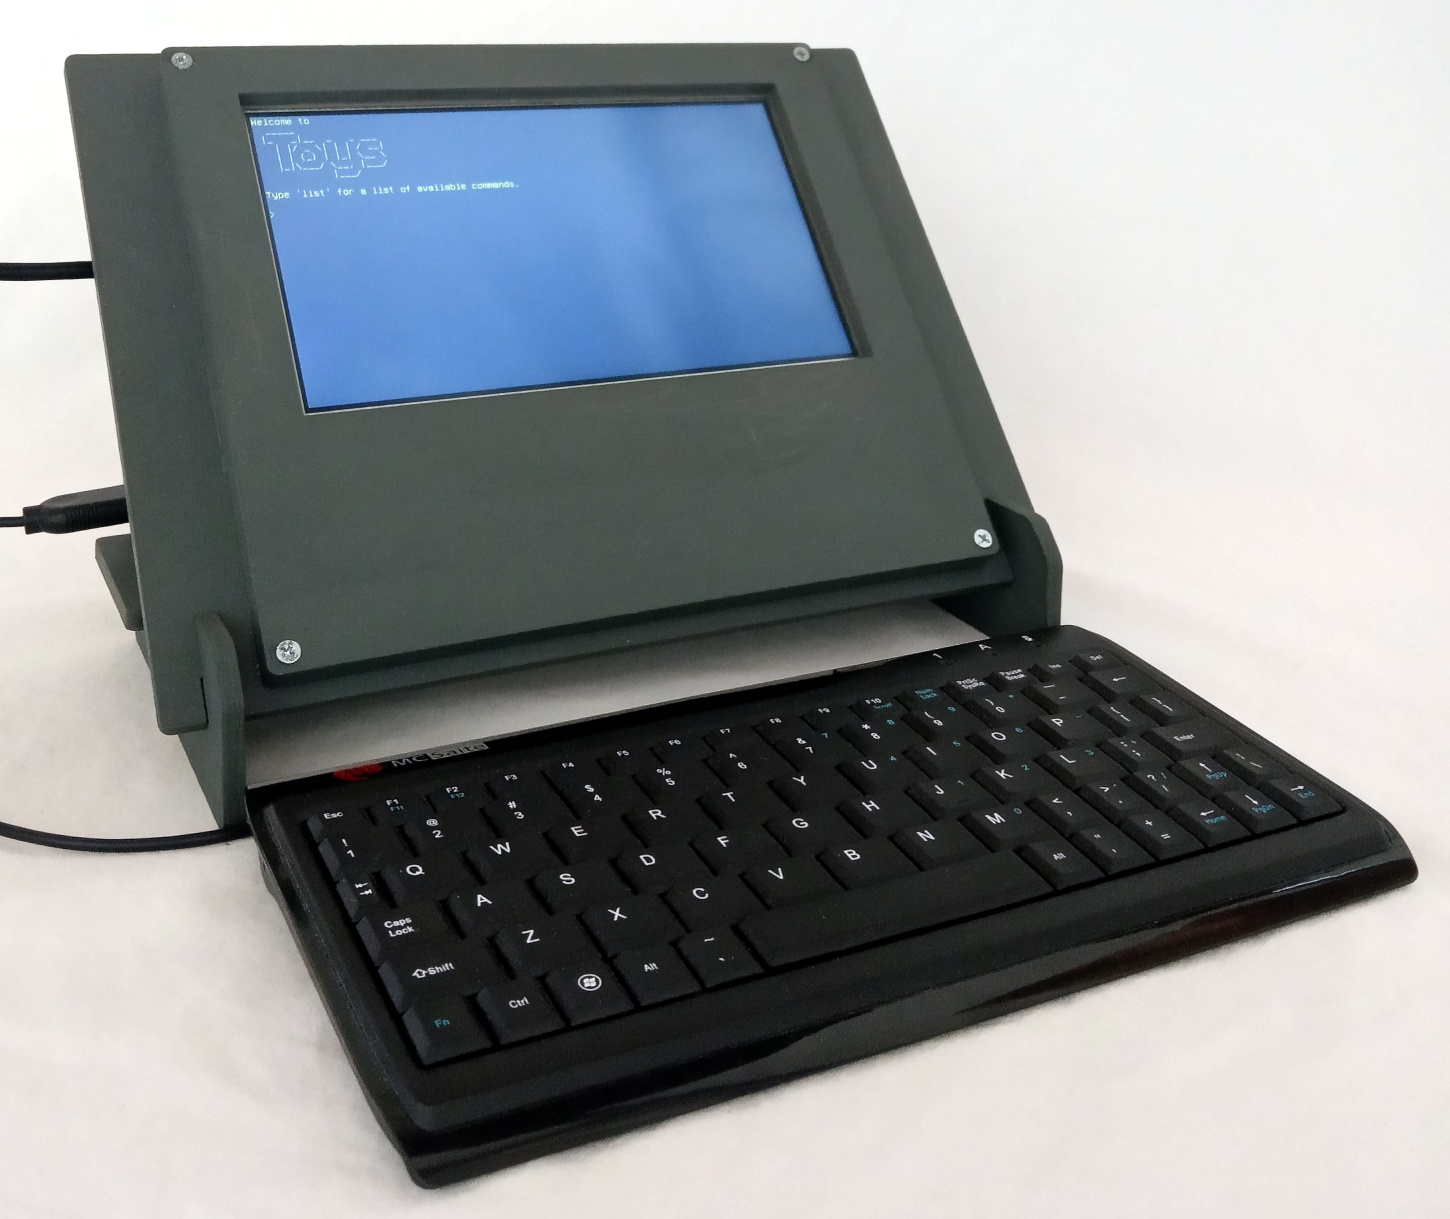
\includegraphics[width=\textwidth]{cover/front}};
\end{tikzpicture}

\end{titlepage}


% This work is licensed under the Creative Commons Attribution NonCommercial
% ShareAlike 4.0 International License. To view a copy of the license, visit
% https://creativecommons.org/licenses/by-nc-sa/4.0/

% Title page -------------------------------------------------------------------

\begin{titlepage}

\begin{flushleft}
\sffamily\fontsize{34}{36}\bfseries\selectfont
Programming\\
a toy computer\\
from scratch

\vspace{12cm}
\fontsize{16}{18}\selectfont
A practical introduction to computer systems\\
\vspace{1cm}
Eric Bruneton
\end{flushleft}
\end{titlepage}

% Copyright page ---------------------------------------------------------------

\thispagestyle{empty}

\vspace*{\fill}

\begin{flushleft}
\textcopyright\ 2024 \, Eric Bruneton

\medskip

\ccbyncsa\ This book is available under the
\href{https://creativecommons.org/licenses/by-nc-sa/4.0/}{Creative Commons
BY-NC-SA 4.0 License}. The programs it contains are also available separately,
under the \href{https://www.gnu.org/licenses/gpl-3.0.en.html}{GNU General
Public License v3}.

\medskip

\textbf{Version} \\ This book was built from commit
\gitcommithash[shortHash=false]\ on \gitcommitdate[formatDate] in the source
code repository. The latest version can be downloaded at \toypcurl{}.

\medskip

\textbf{Source code} \\
The source code of this book, in \href{https://www.latex-project.org/}{\LaTeX}\
and \href{https://www.rust-lang.org/}{Rust}, is available at \\
\url{https://github.com/ebruneton/toypc}. \\
The programs it describes are also available separately, at \\
\toypcurl{}.

\medskip

\textbf{Feedback} \\
Please report errors or potential improvements at \\
\url{https://github.com/ebruneton/toypc/issues}.
\end{flushleft}

\clearpage

% Table of contents ------------------------------------------------------------

\setcounter{tocdepth}{1}
\tableofcontents

\chapter*{Introduction}
\addcontentsline{toc}{chapter}{Introduction}

Billions of people are using computers or smartphones, which are computers
before being phones. One doesn't need to understand how computers work to use
them, but if you want to know, this book might help you.

Popular science books about this topic intentionally leave out many details. On
the other hand, textbooks emphasize theoretical aspects and focus on a narrow
topic. This book is different. Its goal is to introduce how computer hardware
and common programming languages and operating systems work, via a practical
example which can be understood down to the smallest detail.

For this it proposes you to assemble and program your own toy computer. And to
make sure not to omit any details, it explains how you can do this from scratch,
without using any existing programming tool. It is organized in four parts:
\begin{itemize}
  \item the first part briefly presents the main basic ideas used to design
  microprocessors, which are the core component of a computer. This is
  necessary to understand the main concepts used in the next parts. It ends
  with the presentation of a virtual, toy microprocessor, which can be
  simulated online, and of a few programs using it.

  \item the second part explains how the components of your toy computer work,
  how they can be programmed, and how to assemble them. Based on this, it then
  describes how to build a basic system allowing programs to use the computer's
  keyboard and screen. Finally, it presents how an initial program can read and
  execute other programs, based on this input and output system.

  \item the third part explains how a computer can be programmed in a language
  which can be ``easily'' understood by humans, unlike the 0s and 1s used by
  its microprocessor. For this it describes how to progressively build a toy
  language, and a program which can translate it into 0s and 1s that the
  microprocessor can execute. In order to give you an idea of what common
  programming languages look like, this toy language is an extremely simplified
  version of real and popular ones.

  \item the fourth part explains how users can easily store files and launch
  applications on their computer, thanks to a (set of) program(s) called an
  operating system. For this it describes how to progressively build a toy
  operating system for your toy computer. For the same reason as above, this
  system is an extremely simplified version of real, frequently used ones.
\end{itemize}

\subsubsection{Target audience}

This book is designed for people looking for a practical and fully detailed
example introducing how microprocessors, programming languages and operating
systems work. It does not explain the theories and principles behind this. If
you want to learn them, you should read computer science textbooks instead
(some references are provided at the end of each part). Conversely, if you only
want to understand the general ideas, it is better to read popular science
books instead.

\subsubsection{How to read this book}

You can read this book without actually assembling or programming a toy
computer, just to understand how this could be done. In this case you can skip
the tutorial-like sections, which describe concrete steps to follow (plug this
wire here, type this on the keyboard, press this button, etc). This is the
case, in particular, of the ``Experiments'' and ``Compilation and tests''
sections.

Alternatively, you can read this book while following the instructions on an
emulator. In this case you do not need to assemble a toy computer, nor to buy
the necessary components for this (described in \cref{appendix:bom}). Instead,
simply use the emulator provided at \toypcurl{emulator.html}. For this you need
a desktop or laptop computer (tablets and smartphones are not really usable for
this task).

Finally, you can buy the components, assemble them, and follow the instructions
for real. This is more costly but probably more fun than the previous methods.
This method also requires a desktop or laptop computer, with a USB port and
capable of running python3. You can also use all three methods: start with the
first one, then re-read the book with the second method and optionally with the
third, if you feel that you need to (typing a program is slower than reading it
-- this can trigger some questions, and finding the answers yourself can give
you a better understanding).

Note also that, if you are stuck or simply want to skip some steps, you can
follow the instructions of any chapter without doing those of the previous ones
(once the computer is physically assembled, if you choose this method). Hence,
for instance, you can skip the instructions of part 2, do those of part 3 on
the emulator, and those of part 4 for real. You can also already have a look at
the final programs and operating system obtained at the end of this book, on
the emulator, by opening the following link:
\toypcurl{emulator.html?script=backups/final.txt}. See the companion website of
this book for more details (\toypcurl{}).


\mainmatter
\renewcommand\thepart{\arabic{part}}

\part{A Toy Microprocessor}\label{part:processor}

\import{part1/}{part1.tex}

\part{A Basic Input Output System}\label{part:computer}

\import{part2/}{part2.tex}

\part{A Toy Compiler}\label{part:compiler}

\import{part3/}{part3.tex}

\part{A Toy Operating System}\label{part:operating-system}

\import{part4/}{part4.tex}

\renewcommand\thepart{}
\bookmarksetup{startatroot}

\nocite{*}
\bibliographystyle{plain}
\renewcommand{\bibname}{References}
\addtocontents{toc}{\vspace{1cm}}
\bibliography{toypc}

% This work is licensed under the Creative Commons Attribution NonCommercial
% ShareAlike 4.0 International License. To view a copy of the license, visit
% https://creativecommons.org/licenses/by-nc-sa/4.0/

\appendix
\addtocontents{toc}{\protect\appendixintoc}

\chapter{Bill of Materials}\label{appendix:bom}

The table below lists all the necessary components to assemble our toy
computer, with their price as of July 2024. It is important to use the exact
Arduino, display, driver board and keyboard models listed here. Otherwise they
might not work with the programs presented in this book.

Assembling these components requires some soldering tasks. The tools
necessary for this are not included here (you can avoid buying them if you have
access to a makerspace).

\begin{Table}[ht]
  \begin{tabular}{|l|l|}\hline
    \makecell{\thead{Part}} & \makecell{\thead{Net price}} \\ \hline

    \makecell{Arduino Due \\
      Cortex M3 84MHz, 512~KB Flash, 96~KB RAM, 3.3V \\
      \url{https://store-usa.arduino.cc/products/arduino-due}}
    & \$48 \\ \hline

    \makecell{7$^{\prime\prime}$ TFT Display  \\
      800x480 pixels with Touchscreen \\
      \url{https://www.adafruit.com/product/2354}}
    & \$35 \\ \hline

    \makecell{RA8875 Driver Board \\
      for 40-pin TFT Touch Displays - 800x480 max \\
      \url{https://www.adafruit.com/product/1590}}
    & \$40 \\ \hline

    \makecell{Miniature Keyboard \\
      PS/2 and USB interface\\
      \url{https://www.adafruit.com/product/857}}
    & \$30 \\ \hline

    \makecell{4 channel Logic Level Converter \\
      \url{https://www.sparkfun.com/products/12009}}
    & \$4 \\ \hline

    \makecell{Half Sized Breadboard - 400 Tie Points \\
      \url{https://www.adafruit.com/product/64}}
    & \$5 \\ \hline

    \makecell{Male/Male Jumper Wires - 20 x 3$^{\prime\prime}$ (75mm) \\
      \url{https://www.adafruit.com/product/1956}}
    & \$2 \\ \hline

    \makecell{Female/Male Jumper Wires - 20 x 3$^{\prime\prime}$ (75mm) \\
      \url{https://www.adafruit.com/product/1953}}
    & \$2 \\ \hline

    \makecell{\bfseries Total} & \makecell{\bfseries \$166} \\ \hline
  \end{tabular}
  \caption{The Bill of Materials of our toy computer.}\label{table:bom}
\end{Table}

\chapter{ASCII codes}\label{appendix:ascii}

The table below lists the character codes defined by the ``American Standard
Code for Information Interchange'' used in this book. The full list can be
found in \cite{ASCII}.

\begin{flushleft}
  \input{generated/ascii_table.tex}
\end{flushleft}

\chapter{IBM PC Set 2 scancodes}\label{appendix:scancodes}

The table below lists the scancodes which are emitted by each key of the
MCSaite keyboard (see \cref{table:bom}) when it is pressed or released. This is
a subset of the IBM PC Set 2 scancodes
(\url{https://wiki.osdev.org/PS/2_Keyboard#Scan_Code_Set_2}).

\begin{flushleft}
  \input{generated/scancode_table.tex}
\end{flushleft}

\chapter{Compiler error codes}\label{appendix:compilercodes}

The table below gives the meaning of the error codes which can be output by the
compiler implemented in \cref{part:compiler}.

\begin{flushleft}
  \input{generated/error_codes_table.tex}
\end{flushleft}

\chapter{Boot Assistant scripts}\label{appendix:python-scripts}

The following sections list the source code of the scripts used in
\cref{part:computer} on the host computer.

\section{boot\_helper.py}

\bigskip
\input{generated/boot_helper.tex}

\section{flash\_helper.py}

\bigskip
\input{generated/flash_helper.tex}


\backmatter
% This work is licensed under the Creative Commons Attribution NonCommercial
% ShareAlike 4.0 International License. To view a copy of the license, visit
% https://creativecommons.org/licenses/by-nc-sa/4.0/

\thispagestyle{empty}~
\clearpage

\thispagestyle{empty}
\color{white}
\newpagecolor{covercolor}
\newgeometry{
  body={118mm,185mm},
  hcentering,
  vcentering,
  headsep=2pc}

\noindent {\sffamily\fontsize{16}{18}\bfseries\selectfont
Programming a toy computer from scratch}

\bigskip

\noindent This book introduces how computer hardware, programming languages and
operating systems work, via a practical example which can be understood down to
the smallest detail. For this it explains how you can assemble and program a
toy computer, in an entirely bottom-up way, without using any existing
programming tool. The end result is a toy, monotasking operating system with a
command line shell, a text editor, a compiler, and a few utilities, in less
than 3300 lines.

\noindent
\begin{tikzpicture}[overlay]
  \node[anchor=north west,inner sep=0] at (0,-0.5cm)
  {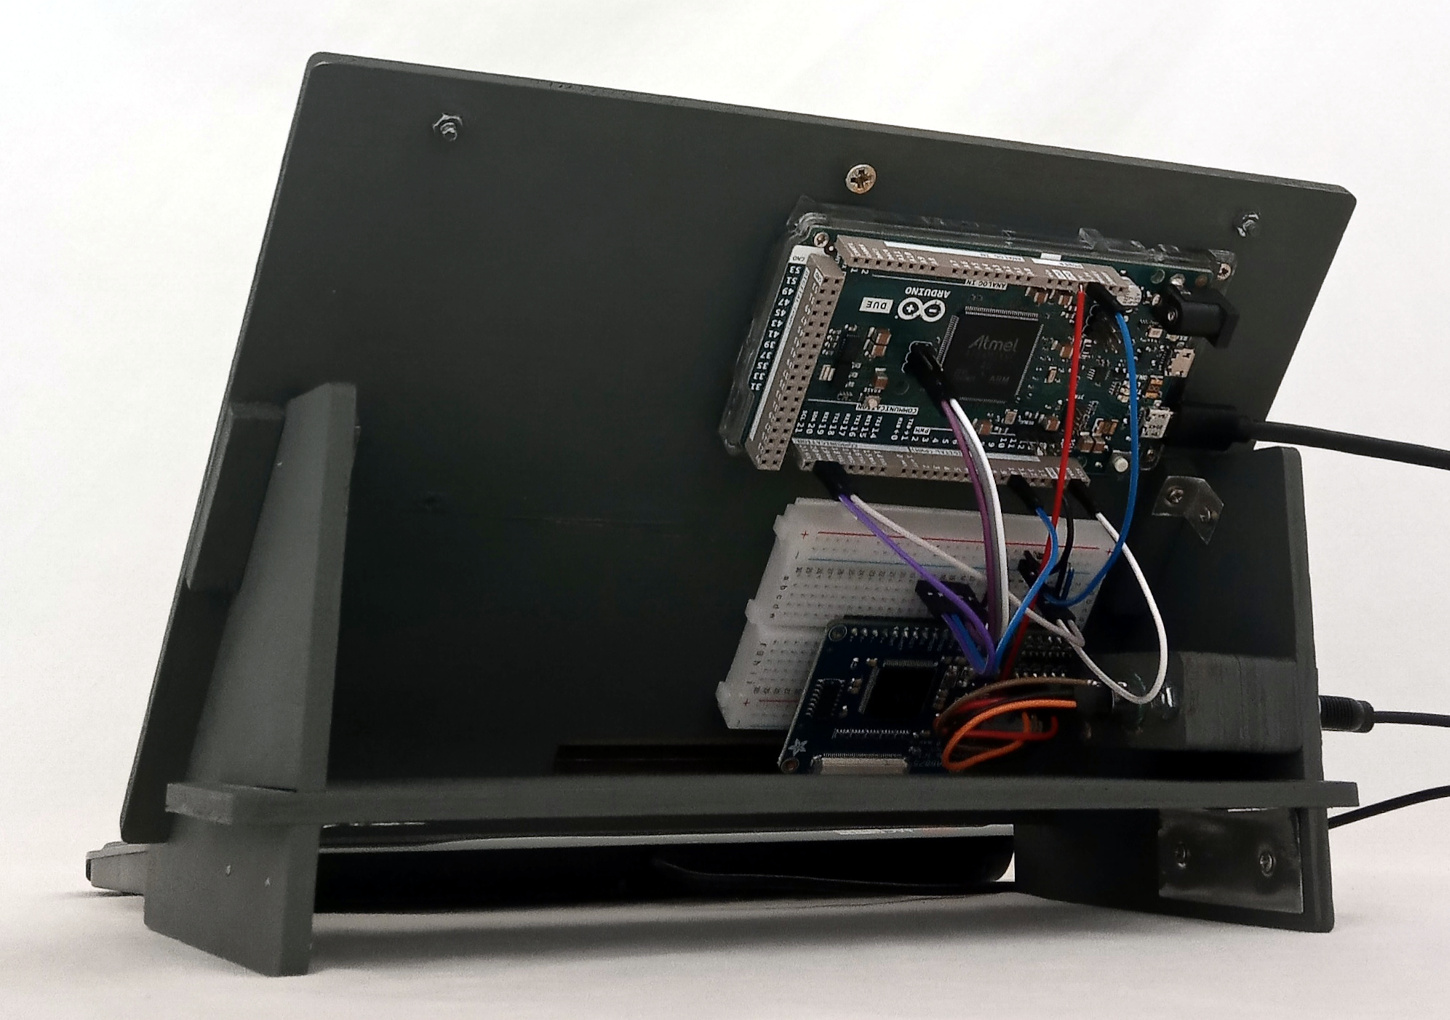
\includegraphics[width=\textwidth]{cover/back}};
\end{tikzpicture}



\end{document}
